\section{Proyecto Final de Unidad - Sistema de Biblioteca} 
\begin{flushleft}

\begin{itemize}
\textbf{1.Antecedentes o introducción}\\
\textbf{ }\\

La palabra Bot proviene de la palabra Robot y es la forma como se le denomina en el lenguaje tecnológico que realiza un procedimiento de manera automática en distintos contextos.
Es un concepto que existe hace casi 50 años, pero con las nuevas herramientas y posibilidades que brinda la época actual, está ganando popularidad dada las diversas aplicaciones que tiene en el mercado.\textbf{ }\\
\textbf{ }\\

Existen varios tipos de Bots, acá nombraremos algunos de los más conocidos: \textbf{ }\\
\textbf{ }\\
•	Bots de seguimiento en redes sociales (Following Bots)\textbf{ }\\
•	Bots de tráfico para sitios web (Traffic Bots)\textbf{ }\\
•	Bots Informativos\textbf{ }\\
•	Bots de conversación (ChatBots)\textbf{ }\\
\textbf{ }\\
El servicio al cliente en redes sociales está cada día más en tendencia, tenemos claro que es más fácil avisar de la falla en algún servicio en redes sociales que llamar y esperar minutos a ser atendido por una operadora.\textbf{ }\\
Es biológicamente imposible que un ejecutivo telefónico pueda atender a más de una persona a la vez por lo que las redes sociales y los canales de comunicación de Internet, tales como chat, correo electrónico, o servicios de mensajería móvil son el conducto ideal para atender a más clientes de forma simultánea, ya que un único ejecutivo puede atender 5 o más personas a la vez.\textbf{ }\\
Si a esta ventaja en atención al cliente le agregaremos bots de primer nivel podemos atender hasta 4 veces más personas que por teléfono con los beneficios adicionales de operar 24/7 todos los días del año.\textbf{ }\\
La idea de tener un bot es complementar la atención humana, haciéndola más eficiente. Apoyar con preguntas frecuentes, consultas simples o tomar datos de manera automática son algunos de los casos más comunes donde se puede aplicar esta tecnología.\textbf{ }\\
\textbf{ }\\
\textbf{2.	Titulo}\\
•         Sistema de Biblioteca
\textbf{ }\\
\textbf{ }\\
\textbf{3.	Autores}\\
•	Acosta Ortiz, Orlando \textbf{ }\\
•	Zegarra Reyes, Roberto\textbf{ }\\
•	Mamani Maquera, Jorge Luis\textbf{ }\\
•	Rivas Rios, Marko\textbf{ }\\
•	Catari Cabrera, Yofer Nain\textbf{ }\\

\textbf{ }\\

\textbf{4.	Planteamiento del problema}\\
\textbf{4.1. 	Problema}\\

Dificultades en la recepción de clientes para realizar ventas o prestamos de libros y atencion a mensajeria online en redes sociales.\textbf{ }\\
\textbf{ }\\
\textbf{ }\\
\textbf{ }\\
\textbf{4.2.	Justificación }\\

La propuesta de nuestro proyecto es mejorar la venta o prestamos de libros al cliente por ende incorporaremos un asistente virtual y permitir brindarle recomendaciones de libros similares. 
\textbf{ }\\
\textbf{4.3.	Alcance }\\
Público en General


\textbf{ }\\
\textbf{5.      Objetivos}\\
\textbf{5.1.   General}\\
-	Poder recomendar diferentes libros a fines al gusto del cliente como podría ser: Autor, Genero, Editorial etc.
\begin{center}
	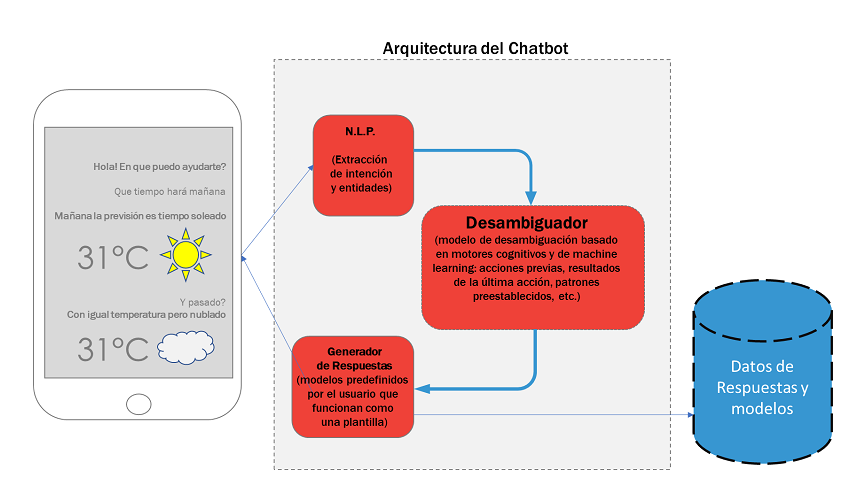
\includegraphics[width=12cm]{./Imagenes/chatbot} 
	\end{center}

\textbf{ }\\

\textbf{5.2.   Específicos}\\

-	Recomendar Libros\\
-	Identificar los gustos literarios del cliente.\\



\textbf{ }\\

\textbf{6.      Referentes teóricos}\\
\textbf{ }\\
\textbf{7.      Desarrollo de la propuesta}\\

\begin{center}
	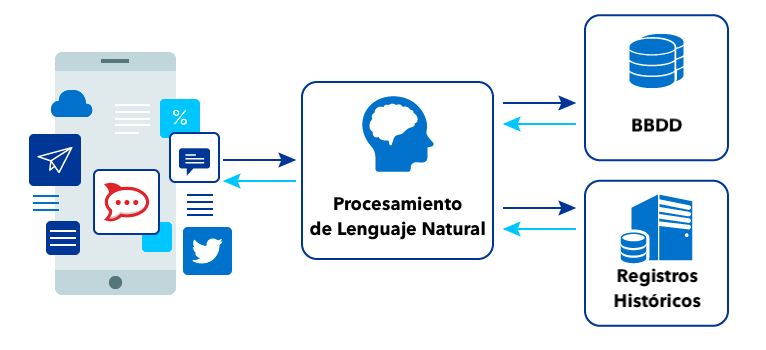
\includegraphics[width=12cm]{./Imagenes/nlp} 
	\end{center}
\textbf{7.1.   Tecnología de información}\\
-	Descripción de productos hardware y software.\\ 
\textbf{ }\\

•	PC core i7 7ta generación, Ram 8GB \\
•	Android \\
•	Visual Code\\
•	MongoDB o MYSQL\\
Funcionalidad de Chatbots( Aquitectura)
\begin{center}
	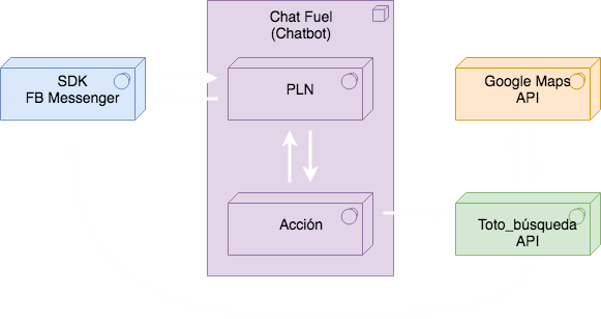
\includegraphics[width=12cm]{./Imagenes/api} 
	\end{center}

\textbf{ }\\
\textbf{7.2.   Metodología, técnicas usadas }\\
-	 desarrollo ágil, la metodología Scrum define perfectamente qué es el método ágil en la gestión de proyectos.
\textbf{ }\\
\textbf{8.      Cronograma (personas, tiempo, otros recursos) }\\
\textbf{ }\\

\textbf{ }\\
\begin{center}
	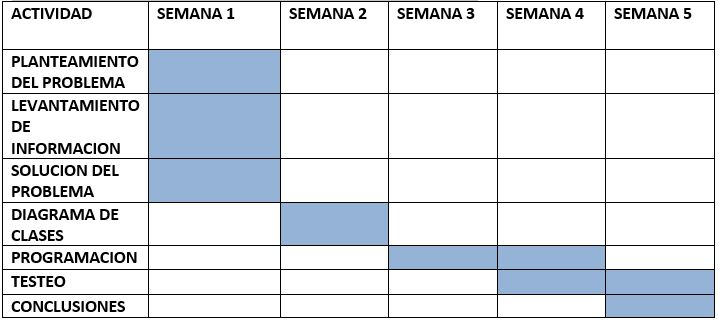
\includegraphics[width=12cm]{./Imagenes/bot1} 
	\end{center}
\textbf{ }\\
\textbf{ }\\
\textbf{ }\\
\textbf{ }\\
\textbf{9.      Presupuesto (Beneficio / Costo, VAN) }\\
\textbf{ }\\
\textbf{ }\\
\begin{center}
	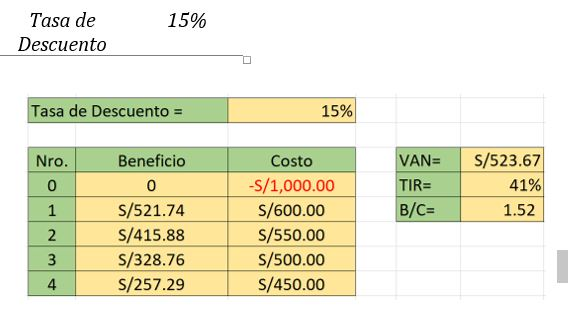
\includegraphics[width=12cm]{./Imagenes/bot2} 
	\end{center}
\textbf{ }\\

\textbf{10.  Conclusiones y Recomendaciones (comentar dificultades y retos en el desarrollo del trabajo)}\\
\textbf{ }\\
-	En la actualidad es necesario contar con este tipo de tecnología ya que mejora la experiencia del usuario por otro lado también nos lleva a recurrir a múltiples tecnologías.\textbf{ }\\
-	Hoy en día el uso de los asistentes virtuales es una herramienta muy importante de interacción porque gracias a ella existe una nueva forma de interactuar con los demás. De esta manera se hace patente la relación entre la tecnología y las personas.\textbf{ }\\


\end{itemize} 


\end{flushleft}